\documentclass[12pt]{beamer}
\usetheme{default} 

\setbeamertemplate{navigation symbols}{} %gets rid of navigation symbols
\setbeamertemplate{footline}{} %gets rid of bottom navigation bars
\setbeamertemplate{footline}[page number]{} %use this for page numbers

\setbeamertemplate{footline}{%
  \raisebox{5pt}{\makebox[\paperwidth]{\hfill\makebox[10pt]{\scriptsize\insertframenumber~~}}}}

\setbeamertemplate{itemize items}[circle] %round bullet points
\setlength\parskip{10pt} % white space between paragraphs

\usepackage{wrapfig}
\usepackage{subfig}
\usepackage{setspace}
\usepackage{enumerate}
\usepackage{graphicx}
\usepackage{amsmath}
\usepackage{amsfonts}
\usepackage{amssymb}
\usepackage{amsthm}
\usepackage[UKenglish]{isodate}
\usepackage{tikz}
\usepackage{pgfplots}
\usepackage{natbib}
\usepackage{hyperref}
\hypersetup{
    colorlinks=true, 
    urlcolor=blue
}
\def\checkmark{\tikz\fill[scale=0.4](0,.35) -- (.25,0) -- (1,.7) -- (.25,.15) -- cycle;} 

% allow drawing arrows
\usetikzlibrary{arrows}
\tikzstyle{arrow}=[draw, -latex] 

% bracketing shortcuts
\newcommand{\paren}[1]{\left(#1\right)}
\newcommand{\sqbracket}[1]{\left[#1\right]}
\newcommand{\cbracket}[1]{\left\{#1\right\}}
\newcommand{\abs}[1]{\left\lvert#1\right\rvert}
\newcommand{\norm}[1]{\left\lVert#1\right\rVert}
% set up the argmin operator, argmax
\DeclareMathOperator*{\argmin}{arg\,min}
\DeclareMathOperator*{\argmax}{arg\,max}

\newcommand{\myframe}[1]{\begin{frame} \frametitle{#1}}

% New itemize environment, with spaces
\newenvironment{spaceitemize}
{ \begin{itemize}
    \setlength{\itemsep}{10pt}
    \setlength{\parskip}{0pt}
    \setlength{\parsep}{0pt}     }
{ \end{itemize}                  } 


% the preamble
\title{Day 3, Session 1: Accessing R help}
\author{Jessica Williams-Nguyen and Brian D. Williamson}
\institute{EPI/BIOST Bootcamp 2017}
\date{26 September 2017}

% Start the document
\begin{document}
% The title page
\begin{frame}
\titlepage
\end{frame}

\myframe{Accessing help}
R can be tricky at times --- but one of the most important things to remember (and easiest things to forget) is that if you are having a problem with R programming, someone else has almost surely had the same problem.

Thankfully, there are a wide variety of resources for getting help with R. These fall into two general categories: \textcolor{blue}{built-in help files} for functions and packages, written by the package maintainers; and \textcolor{green}{online forums} where users can post questions and answers related to programming and/or R.

In addition to being accessed in different ways, parsing the relevant information is somewhat different between these two general categories. 
\end{frame}

\myframe{Help files within R}
To access the help file for a function or package from within R, type \texttt{?} followed by the name of the function you want to learn more about.

For example, if we want to learn about the \texttt{quantile()} function, we type \texttt{?quantile} in the console. This brings up a help page in the file/plot viewer:

\centering
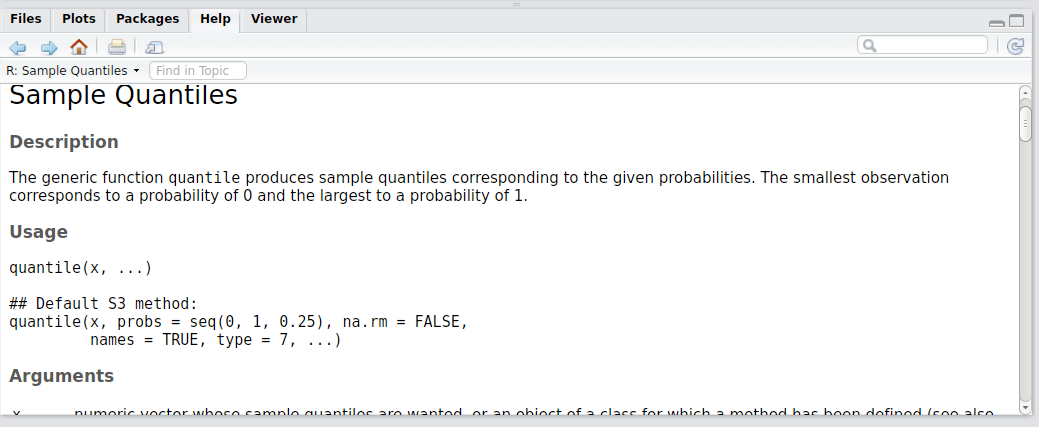
\includegraphics[width = 0.7\textwidth]{figs/help_quantile.png}
\end{frame}

\myframe{Reading R help files}
Help files can be somewhat daunting at first, so learning how to parse out the necessary information is valuable.

Standard R help files consist of a few parts, but the most useful are: the \textcolor{blue}{description}, \textcolor{green}{usage}, \textcolor{purple}{arguments}, \textcolor{brown}{details}, \textcolor{cyan}{value}, and \textcolor{red}{examples}.

\end{frame}

\myframe{Reading R help files: the description}
The first place you should go in an R help file is the description. 

This tells you what the function is supposed to do, and often gives some detail about what you should expect the output to be.

The description is most useful if you see a new function and want to know what it does, or download a new package and want to learn about the functions inside it.

Example: \texttt{?quantile}

\centering
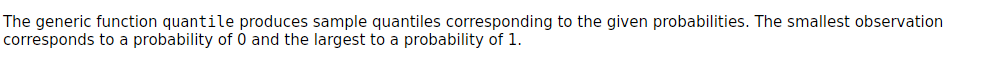
\includegraphics[width = 0.9\textwidth]{figs/description.png}
\end{frame}

\myframe{Reading R help files: usage}
The usage section starts the meat of the help file. Here we learn \textcolor{green}{how to call the function}, and get an introduction to the arguments that it takes (these are described fully in the \textcolor{purple}{arguments} section).

Often, this includes the bare minimum required by the function (the first line), as well as all of the arguments specific to that function (usually called \texttt{Default S3 method}). The default shows you what will happen if you only specify the argument(s) in the first line.

Example: \texttt{?quantile}

\centering
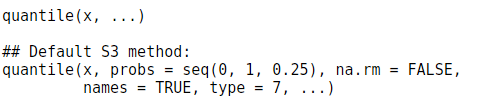
\includegraphics[width = 0.9\textwidth]{figs/usage.png}

\end{frame}

\myframe{Reading R help files: arguments}
Arguments \textcolor{purple}{control behavior of the function}. The most basic argument to a function is the data that it operates on. Other arguments control things like $x$- and $y$-axis labels for plots, or which sample quantile to display, among many other options.

The arguments section tells you how to customize the output of the function to your specifications. 

Example: \texttt{?quantile}

\centering
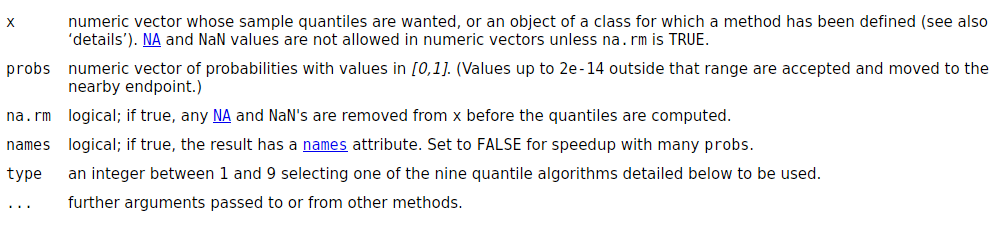
\includegraphics[width = 0.9\textwidth]{figs/arguments.png}
\end{frame}

\myframe{Special argument: ellipsis}
The ellipsis argument \texttt{...} allows arguments to be passed to other functions. This allows the programmer to use functions within their own function, but not specify how the user should customize those other functions.

In the \texttt{quantile()} function, the ellipsis isn't very helpful. However, in the \texttt{hist()} function (which plots a histogram), the ellipsis lets us specify how to set up the plot: we can control things like size of label text relative to the plot and the amount of white space in the margins, among other things.
\end{frame}

\myframe{Reading R help files: details}
The details section often tells us \textcolor{brown}{what certain arguments lead to} when calling the function. This is particularly helpful when you encounter unexpected behavior.

Example: \texttt{?quantile}

\centering
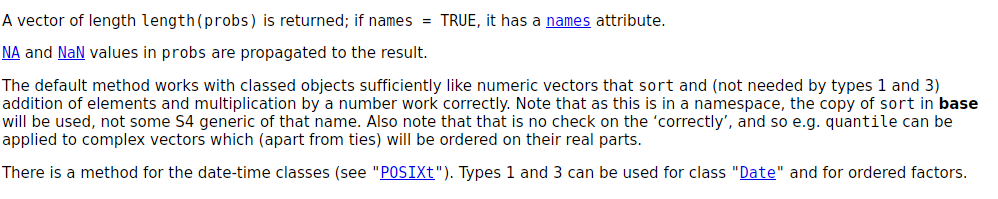
\includegraphics[width = 0.9\textwidth]{figs/details.png}
\end{frame}

\myframe{Reading R help files: value}
The value section tells us \textcolor{cyan}{what the function returns}. This is especially important when you will be taking results from one function and putting them as an argument into a new function!

Example: \texttt{?hist}

\centering
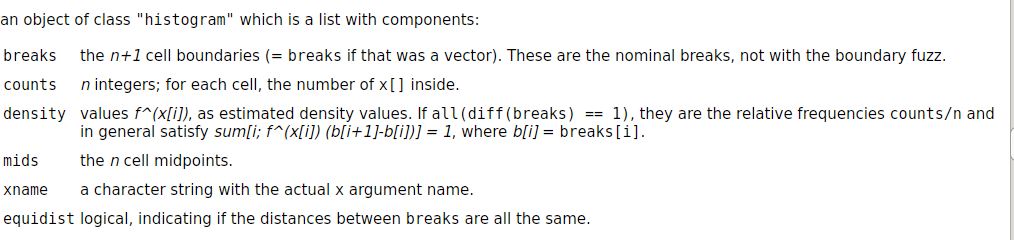
\includegraphics[width = 0.9\textwidth]{figs/value.png}
\end{frame}

\myframe{Reading R help files: examples}
Look here for \textcolor{red}{how to use the function}. Often the examples will be simple, but are good enough to get a rough idea of how the function works.

Example: \texttt{?quantile}

\centering
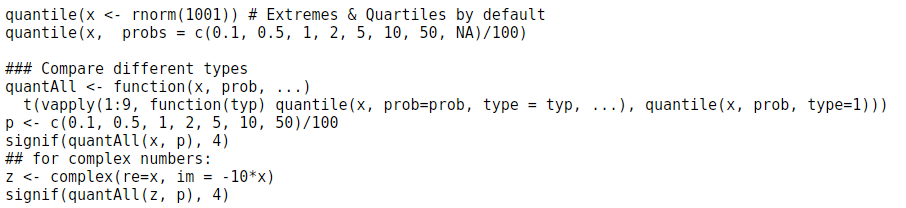
\includegraphics[width = 0.9\textwidth]{figs/examples.png}
\end{frame}

\myframe{Reading R help files: on CRAN}
All R packages that are hosted on CRAN are required to also have a pdf containing all of the help files for the package.

I find this mostly useful to find out what a new package does; these documents can be easily accessed by searching for ``some package CRAN'' (replace ``some package'' with the package name).
\end{frame}

\myframe{Vignettes}
Many R packages now come packaged with \textcolor{blue}{vignettes} --- these are essentially extended examples, which walk you through how to use a particular package or function.

Vignettes can be especially useful for complex functions, like the \href{https://cran.r-project.org/web/packages/dplyr/vignettes/dplyr.html}{one for dplyr} (a useful tool for reshaping data).

If you are new to a particular function, going through the vignette can help you get on your feet quickly!
\end{frame}

\myframe{Useful online resources}
Looking up a help file from within R presumes that you know the name of the function, which sometimes is too much to ask.

A wide variety of problems can lead you to online resources. Often, I go looking for things that I should be able to do in R, but I don't know the exact function name. I also typically research error messages that pop up unexpectedly.

The first resource I always use is Google. Here I will type something like ``do something in R'', which usually brings me to a place like stackoverflow or stackexchange.

These two sites have a wide variety of useful exchanges between people who post questions and answers, and often have exactly the information you need.
\end{frame}

\myframe{Using online resources}
Online resources are great in two respects: typically someone has already asked the question that you have, and typically there are a wide variety of answers to solve the problem; and users can upvote good answers, so that you typically only see the ``best'' answer to a given problem.

However, sometimes there is a difference of opinion on what ``best'' means in a given context --- use your own judgment!

For the most part, you can't go wrong with answers that have received a decent number of upvotes. But keep on scrolling until you find the answer that best matches your particular question!
\end{frame}



\end{document}